\documentclass[a4paper,12pt, twoside]{article} 
\usepackage[french]{babel}
\usepackage[utf8]{inputenc}
\usepackage{answers}

\usepackage{hyperref}

\usepackage[table,xcdraw]{xcolor}
\usepackage{listings}
\definecolor{ForestGreen}{RGB}{34,139,34}

\usepackage{multicol}

\usepackage{enumitem}

\newcommand{\py}{\lstinline{Python} }

%%%%%%%%%%%%%%%%%%%%%%%%%%%%%%%% CONSTANTES %%%%%%%%%%%%%%%%%%%%%%%%%%%%%%%%%%%
\newcommand{\numero}{3}                                    %Numéro de la série -1
\newcommand{\titreserie}{Fonctionnent du système de fichier}  

\definecolor{backcolour}{rgb}{0.95,0.95,0.92}

\lstset{%
	language         = Python,
	backgroundcolor  = \color{backcolour},
	basicstyle       = \ttfamily, % \upshape\ttfamily,
	keywordstyle     = \bfseries\color{blue}, %\bfseries,
	stringstyle      = \color{magenta},
	commentstyle     = \color{ForestGreen},
	alsoletter = > ,
	morekeywords = {>>>,as,assert,False,None, nonlocal,True, with,yield},
	showstringspaces = false,
	numbers=left,
	stepnumber=1,
	literate={à}{{\`{a}}}1 {é}{{\'e}}1 {è}{{\`{e}}}1 {ê}{{\^{e}}}1 {ç}{{\c{c}}}1 {Ç}{{\c{C}}}1,
}

\newcommand{\itemb}[1]{\item \textbf{#1}}

\usepackage{fancyhdr}  %package pour en-tetes et pied de pages
\usepackage{sectsty} % Permet de faire des modifications de police dans diverses sections des "headings" (cf. modif presentation de la page)
\pagestyle{fancy}       %Style pour en-tetes et pieds de pages
\fancyhead[CO,CE]{\sc Série 4\hspace{0.5mm}}
\fancyhead[RO,LE]{Collège Sismondi}  % LaTeX/TEX define \strut to be an invisible box of width zero that extends just enough above and below the baseline. Cela permet d'augementer légèrement la taille en bas de la box de manière à ce qu'elle soit collée à la ligne.
\fancyhead[LO,RE]{\small\ \textsl{1\textsuperscript{er} année - Informatique}}
\fancyfoot[RO,LE]{2021 - 2022}
\fancyfoot[LO,RE]{\small M.Schiess }
\fancyfoot[CO,CE]{\thepage}

\fancyhfoffset[l]{1.2cm} % le "l" en paramètre permet d'indiquer qu'on ne veut modifier que la marge à gauche.
\renewcommand{\headrule}{{%
		\hrule \headwidth \headrulewidth \vskip-\headrulewidth}}
\renewcommand\footrulewidth{\headrulewidth}
\renewcommand{\footrule}{{%
		\vskip-\footruleskip\vskip-\footrulewidth
		\hrule \headwidth \footrulewidth\vskip\footruleskip}}

\usepackage{tikz}
%-------------------------------------------------------------------------------
%---- Eclairage : en encadré sur fond jaune avec symbole "ampoule" à gauche ----
%-------------------------------------------------------------------------------
\definecolor{coleclairage}{RGB}{255 , 221 , 156}
\definecolor{contoureclairage}{RGB}{255 , 192 , 0}
\newenvironment{eclairage}
{
	\begin{center}%
		\begin{tikzpicture}%
			\node[rectangle, draw=contoureclairage, top color=coleclairage!50, bottom color=coleclairage!140, rounded corners=5pt, inner xsep=5pt, inner ysep=6pt, outer ysep=10pt]\bgroup                     
			\begin{minipage}{0.98\linewidth}
				\begin{minipage}{0.08\linewidth}\centerline{
\includegraphics[scale=1]{../../theorie/Images/Symbole_eclairage.png}}\end{minipage}
				\begin{minipage}{0.89\linewidth}\itshape\footnotesize
				}
				{                		
				\end{minipage}
			\end{minipage}\egroup;%
		\end{tikzpicture}%
	\end{center}%
}

%-------------------------------------------------------------------------------
%---- apprendre : en encadré sur fond jaune avec symbole "ampoule" à gauche ----
%-------------------------------------------------------------------------------
\definecolor{colapprendre}{RGB}{50,205,50}
\definecolor{contourapprendre}{RGB}{34,139,34}
\newenvironment{apprendre}
{
	\begin{center}%
		\begin{tikzpicture}%
			\node[rectangle, draw=contourapprendre, top color=colapprendre!10, bottom color=colapprendre!50, rounded corners=5pt, inner xsep=5pt, inner ysep=6pt, outer ysep=10pt]\bgroup                     
			\begin{minipage}{0.98\linewidth}
				\begin{minipage}{0.08\linewidth}\centerline{
\includegraphics[width=30px]{../../theorie/Images/Symbole_learn.png}}\end{minipage}
				\begin{minipage}{0.89\linewidth}\itshape\footnotesize
				}
				{                		
				\end{minipage}
			\end{minipage}\egroup;%
		\end{tikzpicture}%
	\end{center}%
}


%-----------------------------------------------------------------
%---- Modification présentation de la page: marges de la page ----
%-----------------------------------------------------------------
%\addtolength{\hoffset}{-1in}              % 1
%\addtolength{\voffset}{-1in}              % 2
\addtolength{\oddsidemargin}{-0.1 in} % 3
\addtolength{\evensidemargin}{-1in} % 3
\addtolength{\topmargin}{-1in}       % 4
\addtolength{\headheight}{6pt}       % 5
%\addtolength{\headsep}{-0.2cm}           % 6
\setlength{\textheight}{26cm}    % 7
\setlength{\textwidth}{16.5cm}      % 8
\addtolength{\marginparsep}{0pt}      % 9
\setlength{\marginparwidth}{0pt}   % 10
\addtolength{\footskip}{-1mm}           %11

\setlength{\parindent}{0em}% pas d'indentation


% Customiser le nom des sections
\usepackage{titlesec}
\titleformat{\section}[hang]{\Large \bfseries}{Série \thesection:\ }{0pt}{}

\renewcommand{\familydefault}{\sfdefault} % pour avoir des polices san serif

\newtheorem{Exc}{Exercice}
\Newassociation{correction}{Soln}{mycor}
\renewcommand{\Solnlabel}[1]{\bfseries Ex #1 }
\def\exo#1{%
	\futurelet\testchar\MaybeOptArgmyexoo}
\def\MaybeOptArgmyexoo{
	\ifx[\testchar \let\next\OptArgmyexoo
	\else \let\next\NoOptArgmyexoo \fi \next}
\def\OptArgmyexoo[#1]{%
	\begin{Exc}[#1]\normalfont}
	\def\NoOptArgmyexoo{%
		\begin{Exc}\normalfont}
		\newcommand{\finexo}{\end{Exc} \vspace{3mm}}
	\newcommand{\flag}[1]{}
	\newcommand{\entete}[1]

\newcommand{\getexocompteur}{{\the\numexpr \arabic{Exc}  \relax}}	
	
\newcommand{\eexo}{\vspace{5mm}} % espace pour séparer les exercices

\begin{document}
%		\title{\vspace{-3cm}Série 1}
%		\date{\vspace{-2cm}}
%		\maketitle

\fancyhead[CO,CE]{\sc Série \arabic{section} \hspace{0.5mm}}

\setcounter{section}{\numero}
\section{\titreserie }				
\Opensolutionfile{mycor}[cor_01]

\exo{}[Créer un fichier texte]  ~\\ 
	\begin{enumerate}
		\item 	En réfléchissant aux derniers cours, essayer de calculer la taille que ferait un fichier texte nommé blabla.txt qui contiendrait le texte suivant:
		\begin{lstlisting}[numbers=none]
blablabla
		\end{lstlisting}
		\item Créez un fichier texte nommé blabla.txt en  utilisant un éditeur de texte (par exemple l'éditeur \textit{kate}).
		\item A l'aide de l'explorateur de fichier, lire la taille du fichier texte que vous venez de créer.
	\end{enumerate}
	

	 Le fichier doit contenir le texte "Ceci est mon premier fichier texte". Sauvegarder le fichier dans le dossier utilisateur sous "premier\_fichier\_texte.txt".

\finexo

\exo{}[Arborescence et fichiers]  ~\\ 
Dans moodle à la section 4 (4. Fonctionnement de l'ordinateur), télécharger le fichier "fichiers\_exercice2.zip", puis décompressez-le sur votre ordinateur (faire un clique droit depuis l'explorateur de fichier et choisissez "Extraire ici").\\

Ouvrez le dossier "A\_Trier\_A\_Renommer", ouvrir chaque fichier qu'il contient, renommez-les et déplacez-les dans le bon dossier. Renommez également les dossiers avec des noms corrects.\\

Pour finir, refaire une archive du dossier parent nommée "fichiers\_ exercice2\_corrigé.zip" (clique droit compresser) et la déposez dans moodle dans le devoir "Arborescence exercice 2 corrigée" à la section 4 (4. Fonctionnement de l'ordinateur).\\

\textbf{Questions} (après avoir mis les fichiers à leur bonne place)
\begin{enumerate}
	\item Combien y a-t'il de dossiers dans le dossier Animaux ?
	\item Combien y a-t'il de fichiers dans le dossier Legumes ?
	\item Quelle est la taille de l'image avec des carottes ?
	\item Quelle est l'extension de l'image avec des carottes ?
	\item Quelle est la taille du dossier Fruits ?
	\item Donner l'arborescence depuis le dossier parent.
\end{enumerate}
	\begin{correction}
		~\\ 
		\begin{enumerate}
			\item  Il y les deux dossiers "Mammiferes" et "Oiseaux" directement dans le dossier "Animaux", mais il y encore 3 sous-dossiers dans le dossier "Mammiferes" ("Ferme", "Marin" et Savane").
			\item 4
			\item 175.8 ko
			\item jpg
			\item 943.2 ko
			\item Avec la vue détaillée dans l'explorateur Dolphin, on a
			\begin{center}
				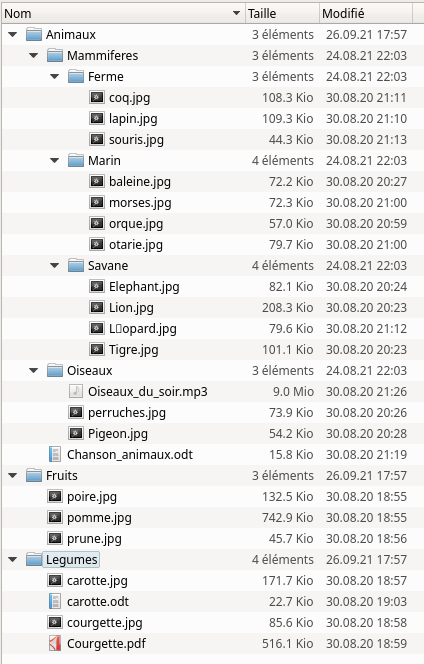
\includegraphics[width=0.6\textwidth]{images/corrige_ex2_tree.png}
			\end{center}

		\end{enumerate}
	\end{correction}
\finexo

\exo{}[Utiliser le Drive]  ~\\ 
	\begin{enumerate}
		\item Se connecter sur www.eduge.ch puis aller sur le drive.
		\item Créer un dossier "Info\_1er" qui contient au moins 3 sous-dossiers appelés:
			\begin{enumerate}
				\item Microbit
				\item Python
				\item Projet
			\end{enumerate}				
	\end{enumerate}
	
	Le prochain petit programme fait en Microbit devra être sauvegardé sur le drive dans le dossier Microbit avec un nom parlant. 

\finexo

\newpage

\exo{}[Format de fichier]  ~\\ 
\begin{enumerate}
	\item Créer un fichier texte contenant le texte suivant:
	\begin{lstlisting}[numbers=none]
P1
21 18
000000010000000001000
000000101000000010100
000001000100000100010
000001000111111100010
000010000000000000001
000010000000000000001
000010000100000100001
000010000000000000001
000010000000100000001
000001000001010000010
000000100000000000100
000011011000000011000
001100000111111100000
010000000100000100000
100000000100000100000
100000000100000100000
101111100100100100000
100000010100100100000
011111100011011000000
	\end{lstlisting}
	\item Ouvrir le fichier depuis l'explorateur de fichiers Dolphin. Quel type d'information contient ce fichier?
	\item Quelle est la taille de ce fichiers en bit.
	\item Utiliser  l'explorateur de fichiers pour connaître la taille du fichier.
\end{enumerate}
\begin{correction}
	~\\
	\begin{enumerate}
	\item Utiliser le logiciel \textit{kate} puis sauvegarder au bon emplacement.
	\item On remarque que c'est une image
	\item Il y a 
	\begin{itemize}
	    \item 21x18 caractère "0 ou 1" donc 378 octets
	    \item 7 caractères de méta-donnée "P1" et "21 18" donc 7 octets
	    \item 21 "retour à la ligne" (2 caractères ascii LF et CR, dépend du codage du fichier parfois seulement 1 caractère) don 44 octets.
	\end{itemize}
	Ce qui fait 378 + 7 + 42 = 427 octets, donc $427\cdot 8 =  3416$ bits.
	\item On devrait retrouver le même nombre.
\end{enumerate}
	
\end{correction}

\finexo

\exo{}[Faire une arborescence]  ~\\ 
Classer, sous la forme d’une arborescence, les fichiers suivants :
\begin{itemize}
	\item des photos de vacances,
	\item des photos de sa classe,
	\item une page de tableur présentant ses notes du trimestre,
	\item des pages de Wikipédia présentant des informations utiles pour son TPE,
	\item des copies de mails personnels,
	\item un fichier texte contenant les notes prises dans une réunion préparatoire au conseil de
	classe,
	\item des fichiers de musique pour son baladeur,
	\item des fichiers de musique téléchargés en préparation de son TPE.
\end{itemize}

	\begin{correction}
	~\\ 
		On commence par donner un nom à chacune de ces catégories, par exemple : photos de vacances, photos	de classe, etc. On peut regrouper les dossiers contenant les photos de vacances, les mails personnels et les fichiers pour son baladeur, dans un dossier Perso, les photos de la classe et les notes prises en réunion dans un dossier Délégué , puisque ces différentes informations sont liées à cette fonction, les pages de Wikipédia et la musique téléchargée pour le TPE peuvent	être rassemblées dans un dossier TPE , enfin on peut regrouper le dossier Délégué, le dossier TPE et les notes du trimestre dans un dossier Pro. On obtient alors l’arborescence suivante.
		
		\begin{center}
			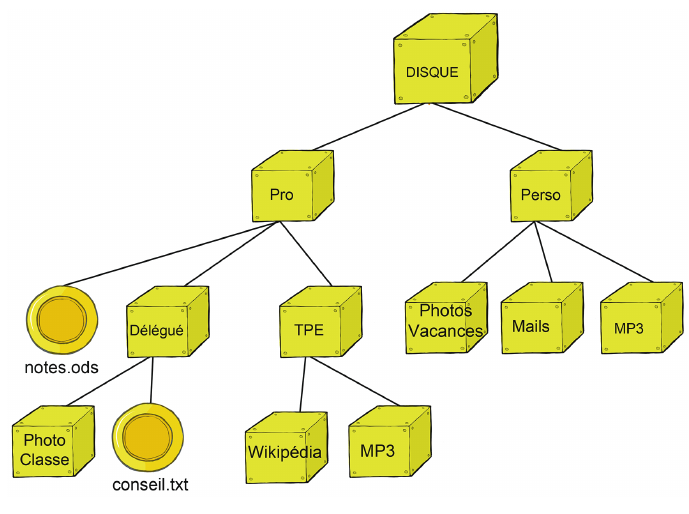
\includegraphics[width=0.6\textwidth]{images/corrige_ex_maketree.png}
		\end{center}

\end{correction}

\finexo

\cleardoublepage

% Solution		
		\newpage
		\setcounter{page}{1}
		\setcounter{section}{\numero}
		\Closesolutionfile{mycor}
		\titleformat{\section}[hang]{\Large \bfseries}{Corrigé Série \thesection:\ }{0pt}{}
		

		\fancyhead[CO,CE]{\sc Corrigé Série \arabic{section} \hspace{0.5mm}}
		\section{}
		\Readsolutionfile{mycor}
	\end{document}